To close an implementation and to ensure that everything were performed correctly, unit and global tests must be done. The diagram presented in figure \ref{fig:tests} reveal the kind of tests that must be validated. 

\begin{figure}[H]
\centerline{
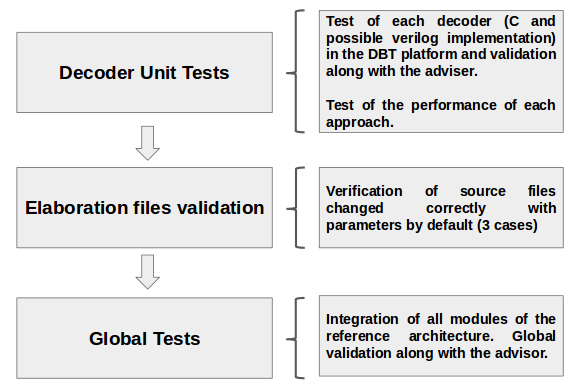
\includegraphics[scale=0.55]{images/tests}
}
\caption{Tests Diagram}
\label{fig:tests} 
\end{figure}

Since one of the goals is to implement the different decoder behaviors, a test to each implementation should be accomplished. If the result is positive, then the integration  of the decode in the DBT is made. Also, performance tests are a goal because it will allow to conclude which behaviors are more efficient. Regarding the implementations in hardware, the group hopes to test those implementations in the Zybo board.

Being the decoder implementations approved, it is verified if the elaboration files replace the annotations in the sources files correctly, meaning that it is checked if the final source files are generated properly.

In the end, all the modules of the DBT will be integrated and a bunch of tests with different configurations will be done.
